\appendix
\addchap{Anhang}
\refstepcounter{chapter}

\section{Metriken aus dem Entwicklungsprozess}\label{appendix:metrics}

\begin{table}[H]
    \centering
    \begin{tabular}{p{6.5cm}p{8cm}} \toprule
    \textbf{\ac{CLOC}} & Anzahl der geänderten Zeilen im Quellcode. \\
    \multicolumn{2}{p{14.5cm}}{\textit{Wie viele Änderungen passieren in der Codebasis? \newline Wo finden die meisten Änderungen statt?}} \\ \midrule
    \textbf{\ac{CLOC} pro Entwickler} & Anzahl der geänderten Zeilen im Quellcode pro Entwickler. \\ 
    \multicolumn{2}{p{14.5cm}}{\textit{Wie viel Code ändert jeder im Team? \newline  Wer ist wie oft in welchem Modul?}} \\ \midrule
    \textbf{\ac{CLOC} pro Commit} & Anzahl der geänderten Zeilen im Quellcode pro Commit. \\ 
    \multicolumn{2}{p{14.5cm}}{\textit{Wie groß sind die Commits?}} \\ \midrule
    \textbf{Commits} & Gesamtzahl an Commits in einem bestimmten Zeitraum. \\ 
    \multicolumn{2}{p{14.5cm}}{\textit{Wie viel Änderungen wurden im Quellcode vorgenommen?}} \\ \midrule
    \textbf{Commits pro Entwickler} & Gesamtzahl an Commits in einem bestimmten Zeitraum pro Entwickler. \\ 
    \multicolumn{2}{p{14.5cm}}{\textit{Wie viel Änderungen wurden im Quellcode von einem Entwickler vorgenommen?}} \\ \midrule
    \textbf{Kommentare pro Commit} & Anzahl der Kommentare pro Commit. \\ 
    \multicolumn{2}{p{14.5cm}}{\textit{Wer arbeitet zusammen? \newline Wie viel wird zusammengearbeitet?}} \\ \midrule
    \textbf{Pull Requests} & Gesamtzahl an Pull Requests in einem bestimmten Zeitraum. \\ 
    \multicolumn{2}{p{14.5cm}}{\textit{Wird mit Pull Requests gearbeitet? \newline Werden Reviews gemacht?}} \\ \midrule
    \textbf{Gemergte Pull Requests} & Anzahl erfolgreicher Pull Requests in einem bestimmten Zeitraum. \\ 
    \multicolumn{2}{p{14.5cm}}{\textit{Wie oft werden erfolgreiche Änderungen in die Codebasis übernommen?}} \\ \midrule
    \textbf{Abgelehnte Pull Requests} & Anzahl abgelehnter Pull Requests in einem bestimmten Zeitraum. \\ 
    \multicolumn{2}{p{14.5cm}}{\textit{Wie oft werden Änderungen an der Codebasis abgelehnt? \newline Wie klar sind die Erwartungen des Teams an eine abgeschlossene Änderung (\ac{DoD})?}} \\ \midrule
    \textbf{Kommentare pro Pull Request} & Anzahl der Kommentare pro Pull Request. \\ 
    \multicolumn{2}{p{14.5cm}}{\textit{Wer arbeitet zusammen? \newline Wie viel wird zusammengearbeitet?}} \\ \bottomrule
    \end{tabular}
    \caption{Kennzahlen aus dem \ac{VCS}}\label{metrics-table-vcs}
  \end{table}
  
  \begin{table}[H]
    \centering
    \begin{tabular}{p{5cm}p{9.5cm}} \toprule
    \textbf{Burn Down} & Die Anzahl erledigte Arbeit über die Zeit. Liefert einen Richtwert, wo man sich gerade im Sprint befindet, verglichen zum Commitment. \\
    \multicolumn{2}{p{14.5cm}}{\textit{Erfüllt das Team seine Commitments? \newline Plant das Team seine Arbeit realistisch?}} \\ \midrule
    \textbf{Velocity} & Eine relative Messung der Konsistenz erledigter Arbeit über die Sprints. \\
    \multicolumn{2}{p{14.5cm}}{\textit{Wie konsistent arbeitet das Team?}} \\ \midrule
    \textbf{Cumulative Flow} & Zeigt wie viel Aufgaben nach Status dem Team zugewiesen sind über die Zeit. \\
    \multicolumn{2}{p{14.5cm}}{\textit{Gibt es Engpässe oder Schwachstellen im Prozess? \newline Müssen gewisse Abläufe im Prozess optimiert werden?}} \\ \midrule
    \textbf{Lead Time} & Zeit zwischen Start und Abschluss einer Aufgabe, vor allem interessant bei Kanban. \\
    \multicolumn{2}{p{14.5cm}}{\textit{Wie schnell können Aufgaben vom Team erledigt werden? \newline Wie lange dauert die Umsetzung eines neuen Features?}} \\ \midrule
    \textbf{Bug Counts} & Die Anzahl an Bugs über die Zeit. \\
    \multicolumn{2}{p{14.5cm}}{\textit{Wie viele Fehler werden vom Team im Entwicklungsprozess übersehen? \newline Wie viel ungeplante Arbeit kam zum Sprint dazu?}} \\ \midrule
    \textbf{Bug-Erzeugungsrate} & Anzahl Bugs nach Erstellungsdatum. \\
    \multicolumn{2}{p{14.5cm}}{\textit{Wie viele Fehler wurden zu einem bestimmten Zeitpunkt erzeugt?}} \\ \midrule
    \textbf{Bug-Fertigstellungsrate} & Anzahl Bugs nach Erledigungsdatum. \\
    \multicolumn{2}{p{14.5cm}}{\textit{Wie viele Fehler wurden zu einem bestimmten Zeitpunkt beseitigt?}} \\ \midrule
    \textbf{Aufgaben-Volumen} & Ist die Anzahl der Aufgaben und kann der Schätzung gegenübergestellt werden, um die Größe der Aufgaben oder ungeplante Arbeit aufzuzeigen. \\
    \multicolumn{2}{p{14.5cm}}{\textit{Wie viel ungeplante Arbeit kam zum Sprint dazu? \newline Wie groß ist die durchschnittliche Aufgabe? Gibt es Ausreißer?}} \\ \midrule
    \textbf{Aufgaben-Rückfälligkeit} & Zeigt auf, wie oft Aufgaben im Arbeitsablauf rückwärts gehen. \\
    \multicolumn{2}{p{14.5cm}}{\textit{Wie viele Aufgaben werden wieder in einen vorhergehenden Status gesetzt? \newline Gibt es Probleme beim Verständnis der Aufgaben? \newline Wie klar sind die Erwartungen des Teams an eine abgeschlossene Änderung (DoD)?}} \\ \bottomrule
    \end{tabular}
    \caption{Kennzahlen aus dem \ac{PTS}}\label{metrics-table-pts}
  \end{table}
  
  \begin{table}[H]
    \centering
    \begin{tabular}{p{6.5cm}p{8cm}} \toprule
    \textbf{Build-Dauer} & Geschätzte und tatsächliche Dauer der Builds. \\
    \multicolumn{2}{p{14.5cm}}{\textit{Wie lange dauert es ein Software-Artefakt zu erstellen? \newline Wie verändert sich die Dauer der Erstellung eines Software-Artefakts über die Zeit?}} \\ \midrule
    \textbf{Build-Status} & Es können die Anzahl der erfolgreichen und fehlerhaften Builds gegenüber gestellt werden. \\
    \multicolumn{2}{p{14.5cm}}{\textit{Gibt es ein Problem im Freigabeprozess?}} \\ \midrule
    \textbf{Build-Frequenz} & Wie oft wird ein Build ausgelöst. \\
    \multicolumn{2}{p{14.5cm}}{\textit{Wird oft genug ein neues Software-Artefakt erstellt?}} \\ \midrule
    \textbf{Test Reports} & Anzahl erfolgreicher und fehlerhafter Tests, Gesamtdauer der Tests. \\
    \multicolumn{2}{p{14.5cm}}{\textit{Wie lange dauert ein kompletter Testdurchlauf? \newline Gibt es Tests, die optimiert werden müssen? \newline Wie oft werden fehlerhafte Tests in die Codebasis aufgenommen?}} \\ \midrule
    \textbf{Code Coverage} & Wie viel Prozent des Quellcodes ist mit Tests abgedeckt. \\
    \multicolumn{2}{p{14.5cm}}{\textit{Gibt es Module, die nicht oder schlecht getestet sind? \newline Wie sieht die Entwicklung der Testabdeckung über die Zeit aus?}} \\ \midrule
    \textbf{Stresstests oder Benchmarking} & Hier kann das Ergebnisse die unterschiedliche Reports sein. \\
    \multicolumn{2}{p{14.5cm}}{\textit{Ist das Produkt auch noch unter Last verwendbar? \newline Wie verändert sich die Leistung über die Zeit?}} \\ \bottomrule
    \end{tabular}
    \caption{Kennzahlen aus den \ac{CI}- und \ac{CD}}-Systemen\label{metrics-table-cicd}
  \end{table}
  
  \begin{table}[H]
    \centering
    \begin{tabular}{p{5cm}p{9.5cm}} \toprule
    \textbf{CPU Nutzung} & Auslastung der Prozessoren über die Zeit. \\
    \textbf{Heap Size} & Auslastung des Heap über die Zeit. \\
    \multicolumn{2}{p{14.5cm}}{\textit{Arbeitet die Software technisch effizient? \newline Ist die Hardware ausreichend? \newline Gibt es eine erhöhte Auslastung nach einer Änderung?}} \\ \midrule
    \textbf{Fehlerraten} & Anzahl Fehler über die Zeit (kann aus dem Logging kommen). \\
    \multicolumn{2}{p{14.5cm}}{\textit{Werden seit einer Änderung mehr Fehler produziert? \newline Wie entwickelt sich die Fehlerrate über die Zeit?}} \\ \midrule
    \textbf{Antwortzeiten} & Dauer der Verarbeitung bestimmter Anfragen. \\
    \multicolumn{2}{p{14.5cm}}{\textit{Reagiert und arbeitet das Produkt noch schnell genug? \newline Gibt es Geschwindigkeitsprobleme seit der letzten Änderung? \newline Wie entwickeln sich die Antwortzeiten über die Zeit?}} \\ \midrule
    \textbf{Benutzeranzahl} & Anzahl gleichzeitiger Benutzer in der Applikation über die Zeit. \\
    \multicolumn{2}{p{14.5cm}}{\textit{Wie entwickeln sich die Nutzerzahlen mit der Zeit? \newline Geht das Produkt in die richtige Richtung? \newline Ist mit höheren Lasten zu rechnen?}} \\ \midrule
    \textbf{Aufenthaltsdauer} & Verweildauer der Benutzer auf bestimmten Seiten. \\
    \multicolumn{2}{p{14.5cm}}{\textit{Welche Features werden besonders oft / selten genutzt? \newline Hat das neue Feature den gewünschten Effekt? Wird es genutzt?}} \\ \midrule
    \textbf{Conversion Rate} & Anzahl Benutzer die zu Kunden wurden. \\
    \multicolumn{2}{p{14.5cm}}{\textit{Wie entwickelt sich die Zahl der zahlenden Neukunden?}} \\ \midrule
    \textbf{Semantisches Logging} & Strukturierte Daten aus dem Logging. \\
    \multicolumn{2}{p{14.5cm}}{\textit{Hier können Daten zu anderen Fragen gesammelt werden, die für den Prozess wichtig sind.}} \\ \bottomrule
    \textbf{Verfügbarkeit} & Verfügbarkeit der Applikation über die Zeit. \\
    \multicolumn{2}{p{14.5cm}}{\textit{Wie hoch ist die Ausfallsicherheit? \newline Wie lange war die Applikation nicht verfügbar?}} \\ \bottomrule
    \end{tabular}
    \caption{Kennzahlen aus den \ac{APM}- und \ac{BI}}-Systemen\label{metrics-table-apm}
  \end{table}

\newpage
\section{Ergebnisse Analyse Retrospektiven}\label{appendix:retros}

\subsection*{Welche guten Entscheidungen haben wir getroffen?}
\begin{enumerate}
    \item sprint (4)
    \item einblick (3)
    \item onboarding (3)
    \item pair (3)
    \item programming (3)
    \item system (3)
    \item arbeit (2)
    \item daily (2)
    \item erledig (2)
    \item information (2)
    \item issu (2)
    \item po (2)
    \item review (2)
    \item reviewing (2)
    \item schnell (2)
    \item stori (2)
    \item urlaub (2)
    \item angenehm (1)
    \item annehm (1)
    \item cloud (1)
    \item dailys (1)
    \item diskussion (1)
    \item dor (1)
    \item durchgefuhrt (1)
    \item einfach (1)
\end{enumerate}

\subsection*{Was haben wir gelernt?}
\begin{enumerate}
    \item sprint (7)
    \item onboarding (4)
    \item team (4)
    \item arbeit (3)
    \item besprech (3)
    \item board (3)
    \item datenfluss (3)
    \item issus (3)
    \item planungswoch (3)
    \item retro (3)
    \item richtlini (3)
    \item system (3)
    \item uberblick (3)
    \item umgestellt (3)
    \item altlast (2)
    \item analogboard (2)
    \item approved (2)
    \item backlog (2)
    \item daily (2)
    \item digital (2)
    \item direkt (2)
    \item genau (2)
    \item impediment (2)
    \item infrastruktur (2)
    \item iso (2)
\end{enumerate}

\subsection*{Was können wir besser machen?}
\begin{enumerate}
    \item sprint (10)
    \item review (7)
    \item checklist (4)
    \item daily (4)
    \item display (4)
    \item doku (4)
    \item issu (4)
    \item po (4)
    \item einarbeitung (3)
    \item einkalkuli (3)
    \item gross (3)
    \item https (3)
    \item java (3)
    \item stori (3)
    \item ablauf (2)
    \item anderung (2)
    \item arbeitspaket (2)
    \item aufnehm (2)
    \item aufteil (2)
    \item backlog (2)
    \item blocked (2)
    \item dokumenti (2)
    \item erledig (2)
    \item geplant (2)
    \item geschatzt (2)
\end{enumerate}

\subsection*{Was nervt uns noch immer?}
\begin{enumerate}
    \item problem (11)
    \item updat (11)
    \item apis (10)
    \item archiv (10)
    \item erreichbar (10)
    \item infrastruktur (10)
    \item jenkin (10)
    \item test (9)
    \item umgebung (9)
    \item dba (8)
    \item eingerichtet (8)
    \item jndi (8)
    \item laut (8)
    \item verwendbar (8)
    \item arbeit (7)
    \item impediment (7)
    \item iso (7)
    \item lang (7)
    \item mitarbeit (6)
    \item mehr (5)
    \item wichtig (5)
    \item anderung (4)
    \item aufteilbar (4)
    \item gross (4)
    \item klar (4)
\end{enumerate}

\newpage
\section{Umfrage Scrum Team}

\subsection{Fragebogen}\label{appendix:questions}
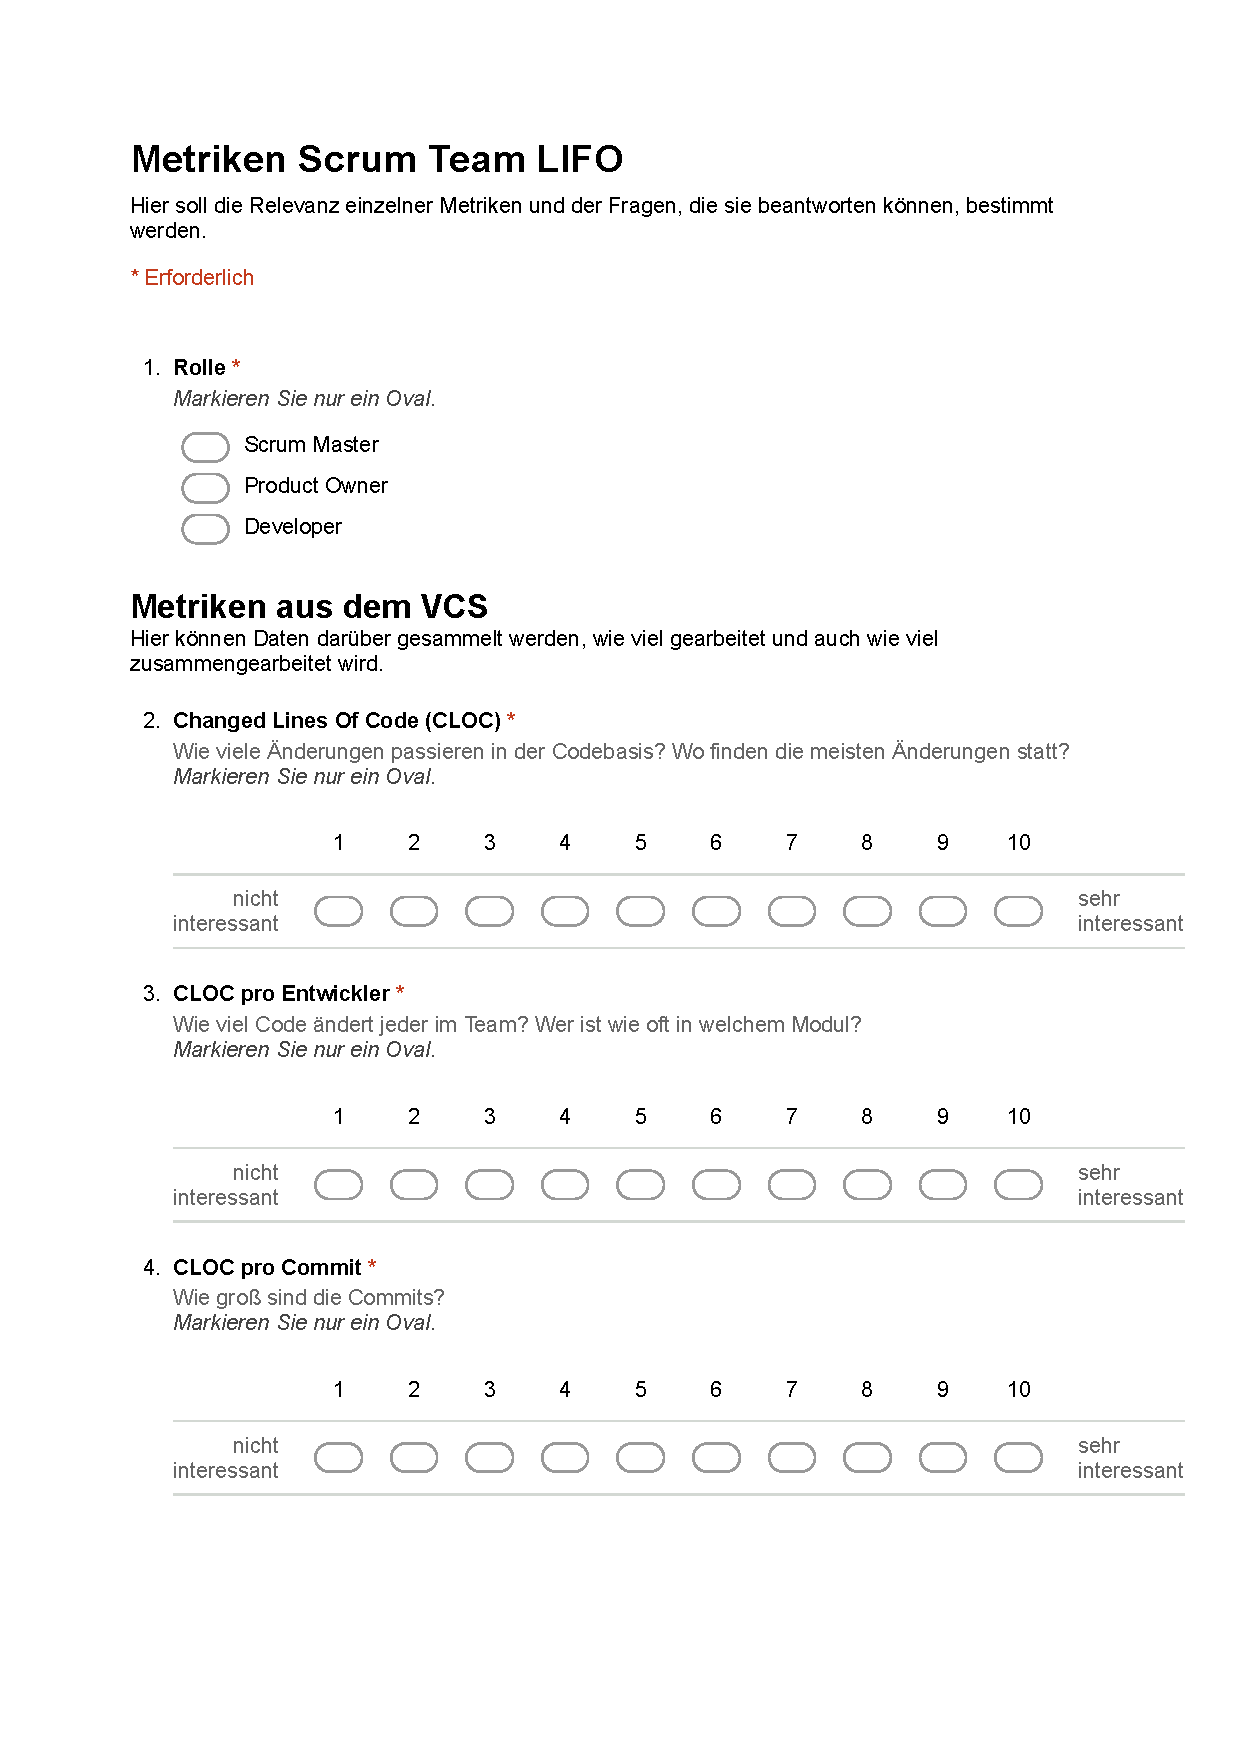
\includepdf[pages=-, scale=0.9, pagecommand={\thispagestyle{plain}}]{appendix/fragebogen.pdf}

\subsection{Ergebnisse}\label{appendix:answers}
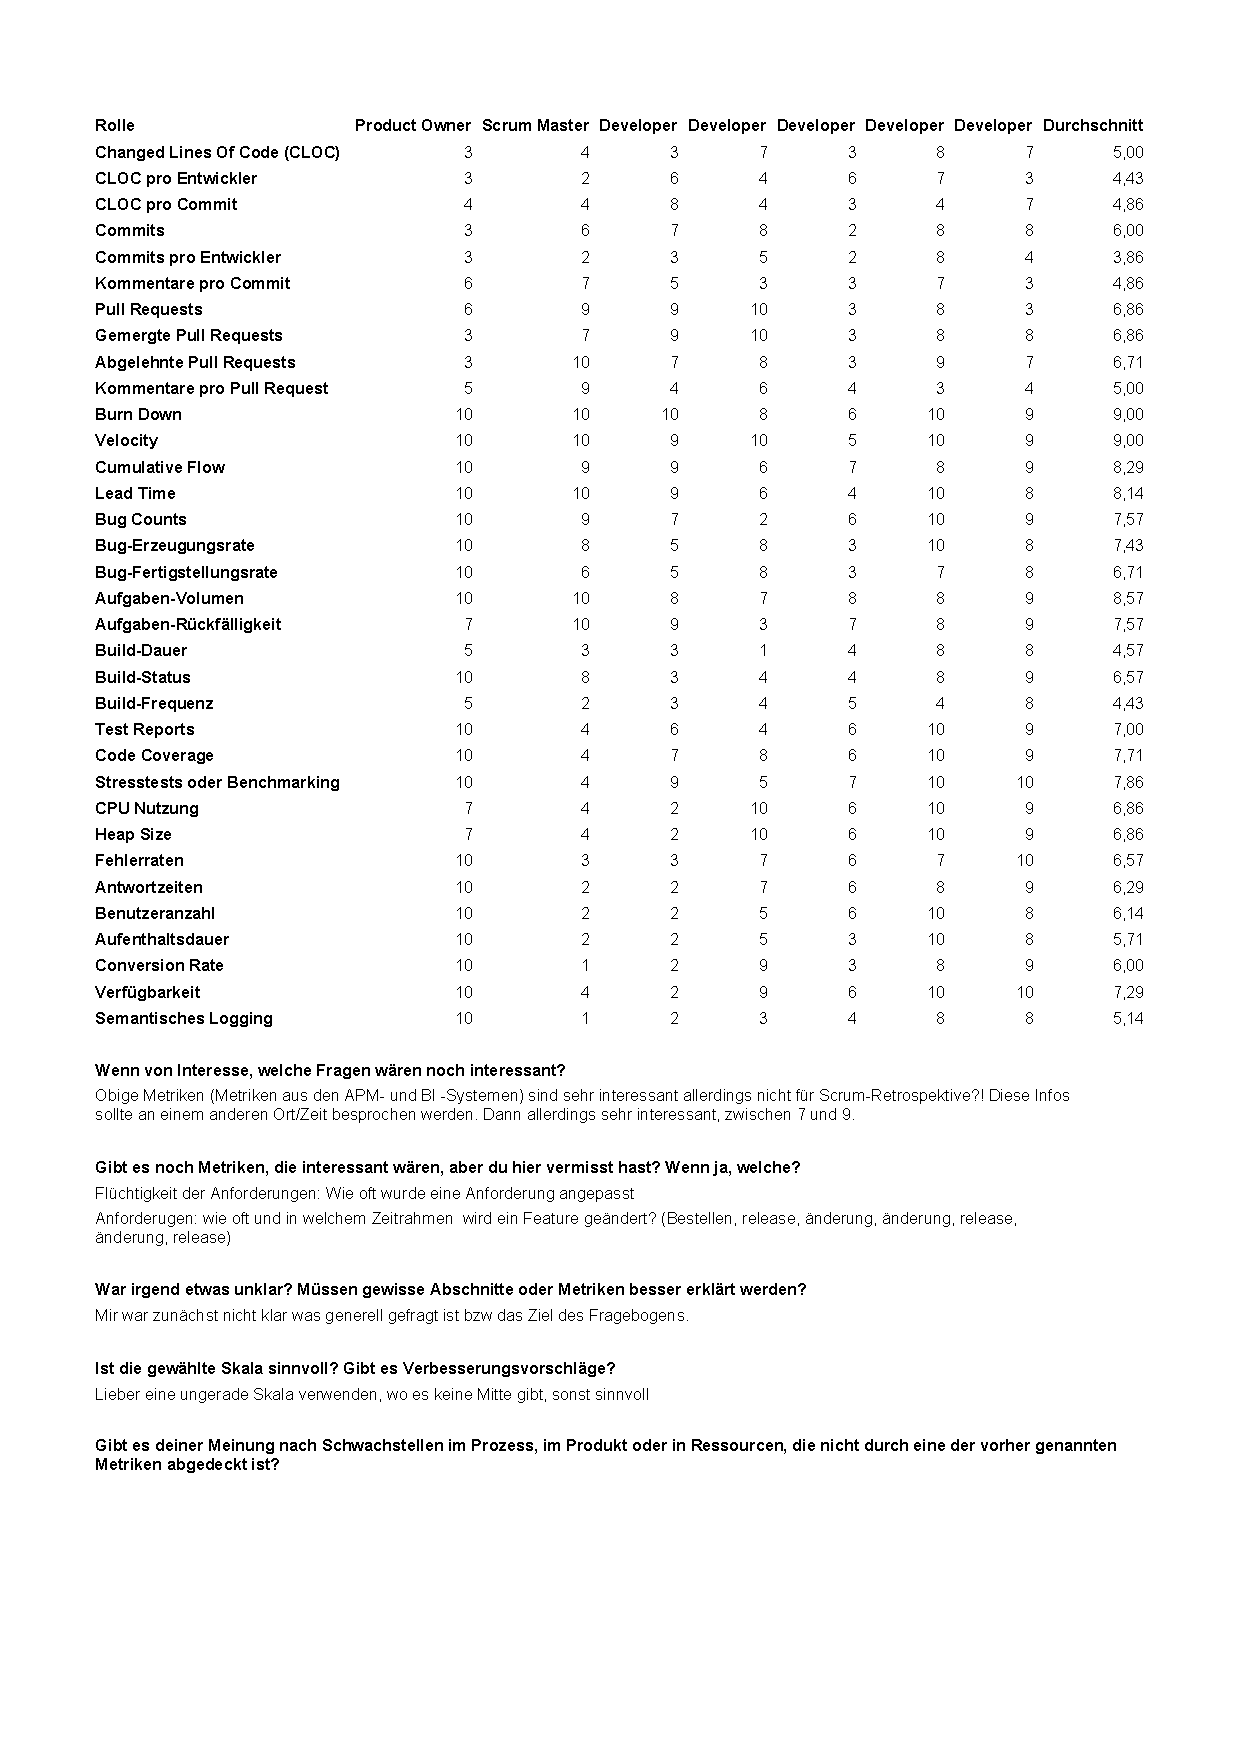
\includepdf[pages=-, scale=0.9, pagecommand={\thispagestyle{plain}}]{appendix/fragebogen-ergebnis.pdf}

\newpage
\section{Transkripte Interviews}\label{appendix:transcript}

Im Folgenden finden sich die Transkripte zu den Interviews, die zu Evaluationszwecken geführt wurden.
Der Interviewer wird mit A und der oder die Interviewte mit B abgekürzt.

\subsection{Product Owner}

A\@: ``Wird das Dashboard von dir genutzt? Wenn ja, wie?'' \\
B\@: ``Bisher primär zur Demonstration, was du in deiner Arbeit gemacht hast. Ich habe es vielen gezeigt, auch darum, um zu zeigen, man kann einfach Daten sammeln und Metriken darstellen. Probleme habe ich teilweise noch mit den Metriken selbst, weil sie nicht alle ausreichend verständlich sind für mich. Uns wären auch noch viele andere eingefallen, beispielsweise zur Darstellung der Testabdeckung der Oberflächentests. Die Herausforderung für die Zukunft wird sein, sinnvolle Metriken finden zu können. Es muss klarer sein, was das Ziel der Metriken ist. Große Probleme hatte ich mit der Acceptance Criteria Volatility. Ich war aufgrund der Zahl irritiert, da ich Prozent gewohnt bin. Diese Metrik muss auch dahingehend verändert werden, dass die Veränderungen erst ab dem Status Prepared gezählt werden, denn davor ist es noch Aufarbeitung der Aufgabe, da kann sich noch viel ändern. Mir war ebenfalls nicht klar, was ist gut, was ist schlecht. Sehr nützlich wäre aus meiner Sicht auch noch eine textuelle Beschreibung der Ziele, die mit den Metriken verfolgt werden. Damit auch in der Retrospektive klar ist, was ist gut gelaufen und was nicht und auch Empfehlungen gegeben werden, wie ein Ziel verbessert werden kann. Ein Beispiel wären die Atlassian Playbooks~\footcite{atlassian_playbook}, die spielerisch versuchen, Probleme im Prozess zu beseitigen.'' \\
A\@: ``Rückblickend gesehen, wurden die richtigen Metriken ermittelt und auf dem Dashboard visualisiert?'' \\
B\@: ``Schwierig zu sagen, für mich ist primär die Acceptance Criteria Volatility interessant, da sie eine Aussage über meine Arbeit trifft. Ein Vorschlag wäre noch, aufzuteilen, für wen welche Metriken interessant sein könnten. Die Einteilung könnte noch etwas klarer sein. Interessant wäre jetzt auch eine Kombination der Metriken, zum Beispiel die Bug Rate kombiniert mit den Releasezyklen. Ich lasse mich überraschen, was der Scrum Master für Ideen hat, weil es grundsätzlich seine Herausforderung sein wird.''

\subsection{Scrum Master}

A\@: ``Ich sehe, du hast schon etwas vorbereitet, du kannst gerne anfangen.'' \\
B\@: ``Ein paar Dinge, die mir aufgefallen sind: Im Dashboard wäre es sehr nützlich, den Zeitraum auf `ab dem letzten Sprint' setzen zu können, das muss jetzt immer manuell als absolutes Datum gesetzt werden. Sinnvoll wäre auch noch, wenn die Generierung der Daten vor Mitternacht passiert, damit sie den Zeitstempel des richtigen Tages haben. Interessant sind auch die Tage, an denen der alte Sprint geschlossen und der neue gestartet wird. Wie es sich dann damit verhaltet. Weiters ist mir noch aufgefallen, dass die Visualisierung bei den Labels nicht sinnvoll ist für unser Team, eine solche Wortwolke ist eher nützlich für das Management, für uns wäre eine Verteilung interessanter, um zu sehen, wie sie sich entwickeln. Bei der Lead Time ist mir aufgefallen, dass ich im Vergleich zum \ac{PTS} noch zu wenig Detailinformationen habe. Für mich sehr nützlich ist die Velocity über die Sprints, weil man sieht, ob sich die geschätzten und erledigten Punkte über eine längeren Zeitraum angleichen. Im \ac{PTS} finden sich noch weitere Metriken, die interessant sein könnten. In Zukunft werden wir auch mit Versionen arbeiten, diese könnten ebenfalls interessant sein im Dashboard, beispielsweise, wie lange wurde an einer Version gearbeitet oder wie viele Entwickler waren beteiligt.'' \\
A\@: ``Wird das Dashboard von dir genutzt? Wenn ja, wie?'' \\
B\@: ``Ich öffne es regelmäßig, für mich sind die Long Term Metrics interessanter, dort betrachte ich meist die letzten 30 Tage, um zu sehen, wie entwickelt sich das Team über die letzten zwei Sprints. Vor allem die Velocity ist hier interessant, eine Trendlinie wäre hier super, um noch besser zu sehen, wie sich die Kennzahlen entwickeln.'' \\
A\@: ``Ist das Dashboard übersichtlich und klar eingeteilt?'' \\
B\@: ``Die Einteilung in Short Term und Long Term Metrics macht auf jeden Fall Sinn, die Anordnung ist für mich okay, mit den Coverage Daten kann ich jetzt weniger anfangen, mit dem Cumulative Flow schon mehr. Wobei wir diesen jeden Tag auf unserem physischen Scrumboard sehen. Kombiniert mit anderen Metriken würde das dann mehr Sinn machen, beispielsweise mit der Bug Rate. Burndown Chart macht in dieser Form auch wenig Sinn, das haben wir im \ac{PTS}, aber auch das macht in Kombination mit anderen Metriken Sinn. Issue Labels könnten als Liniendiagramm dargestellt und in die Long Term Metrics übernommen werden, um Trends erkennbar zu machen. Diese lässt sich dann auch einfacher mit anderen Metriken kombinieren, um Verbindungen herstellen zu können. Sehr interssant sind auch die Aufgaben, die zusätzlich zum Sprint hinzukommen. Generell kann jetzt begonnen werden, gewisse Metriken zu kombinieren, um noch bessere Einsichten in den Prozess zu bekommen.'' \\
A\@: ``Rückblickend gesehen, wurden die richtigen Metriken ermittelt und auf dem Dashboard visualisiert?'' \\
B\@: ``Ja die Metriken sind recht gut gewählt. Je mehr wir sammeln und anzeigen können, desto besser. Aber auch je mehr wir kombinieren können, desto besser.'' \\
A\@: ``Welche Metriken auf dem Dashboard sind besonders nützlich oder werden oft genutzt?'' \\
B\@: ``Für mich sind die Trends in den Long Term Metrics interessanter. Gut wären auch noch detailliertere Ansichten, beispielsweise, wenn ich einen Punkt in einem Diagramm anklicke, dass ich sofort sehe, welche Daten dort dahinter liegen. Derzeit muss ich das dann über das \ac{PTS} ermitteln.'' \\
A\@: ``Ist bereits eine Qualitätsverbesserung im Prozess oder in einem Produkt spürbar? Oder sogar nachweisbar?'' \\
B\@: ``Noch nicht, wir haben es verwendet und alle einmal hinein gesehen, aber momentan ist es noch so, dass wir Daten sammeln, weil mit den zwei oder drei Sprints noch keine klare Aussage getroffen werden kann. Außerdem sind unsere Sprints noch sehr unterschiedlich, wie du sehen kannst.''

\subsection{Entwicklerin}

A\@: ``Wird das Dashboard von dir genutzt? Wenn ja, wann und wie nutzt du das Dashboard?'' \\
B\@: ``Aktuell nutze ich das Dashboard nicht sehr oft, aber wenn ich es nutze, finde ich es sehr hilfreich, dass ich gleich die Code Coverage sehe, so erspare ich mit den Blick ins SonarQube. Auch sehr interessant für mich sind die Anzahl Bugs und zusätzlich aufnehmen könnte man noch die Vulnerabilities aus SonarQube, um den aktuellen Status der Software besser erkennen zu können.'' \\
A\@: ``Ist das Dashboard übersichtlich und klar eingeteilt?'' \\
B\@: ``Aktuell ist die Einteilung für mich klar, ich persönlich würde noch den Cumulative Flow weiter nach unten schieben, da für mich vor allem die Short Term Metrics interessant sind.'' \\
A\@: ``Rückblickend gesehen, wurden die richtigen Metriken ermittelt und auf dem Dashboard visualisiert?'' \\
B\@: ``Ja, in Zukunft kann es noch weiter ausgebaut werden, auch, dass alle Produkte noch detiallierter dargestellt werden.'' \\
A\@: ``Werden Long Term Metrics auch von dir genutzt?'' \\
B\@: ``Interessant finde ich die Velocity, um erkennen zu können, was wir uns vorgenommen haben und was wir wirklich abschließen konnten. Auch die Acceptance Criteria Volatility finde ich sehr interessant, vor allem um den Prozess noch weiter zu verbessern. Hier sind auch die Histogramme hilfreich, um die Verteilung besser erkennen zu können. Für manche war diese Kennzahl verwirrend, da nicht klar war, ob es Prozent sind. Eine bessere Beschreibung wäre hier sinnvoll. Generell werden die Long Term Metrics eher bei den Retrospektiven genutzt.'' \\
A\@: ``Ist bereits eine Qualitätsverbesserung im Prozess oder in einem Produkt spürbar? Oder sogar nachweisbar?'' \\
B\@: ``Mir persönlich ist aufgefallen, dass wir durch den Bug Count frühzeitig gewarnt werden und auch gleich reagieren können.'' \\
A\@: ``Gibt es aus deiner Sicht Verbesserungspotential? Wo liegen aus deiner Sicht die Schwächen dieser Lösung?'' \\
B\@: ``Was mir noch nicht ganz klar ist, bei der Coverage, auf welchen Branch sich das bezieht.'' \\
A\@: ``Die SonarQube Komponente kann bei der Erstellung des Diagramms angegeben werden, in diesem Fall der Master Branch.'' \\
A\@: ``Rückblickend gesehen, wurden die richtigen Metriken ermittelt und auf dem Dashboard visualisiert?'' \\
B\@: ``Ich finde die Short Term Metrics sehr gut gewählt, wie schon gesagt, vermisse ich hier noch die Vulnerabilities aus SonarQube, zumindest für die wichtigsten Komponenten.''
